% Unofficial University of Cambridge Poster Template
% https://github.com/andiac/gemini-cam
% a fork of https://github.com/anishathalye/gemini
% also refer to https://github.com/k4rtik/uchicago-poster

\documentclass[final]{beamer}

% ====================
% Packages
% ====================

\usepackage[T1]{fontenc}
\usepackage{lmodern}
\usepackage[orientation=portrait,size=a0,scale=1.0]{beamerposter}
\usetheme{gemini}
\usecolortheme{nott}
\usepackage{graphicx}
\usepackage{booktabs}
\usepackage{tikz}
\usepackage{pgfplots}
\pgfplotsset{compat=1.14}
\usepackage{anyfontsize}
\usepackage{ragged2e}
\let\olditem\item
\renewcommand\item{\olditem\justifying}

% ====================
% Lengths
% ====================
\bibliographystyle{unsrt}
% If you have N columns, choose \sepwidth and \colwidth such that
% (N+1)*\sepwidth + N*\colwidth = \paperwidth
\newlength{\sepwidth}
\newlength{\colwidth}
\setlength{\sepwidth}{0.025\paperwidth}
\setlength{\colwidth}{0.45\paperwidth}

\newcommand{\separatorcolumn}{\begin{column}{\sepwidth}\end{column}}
\setbeamertemplate{itemize/enumerate subbody begin}{\large}
\setbeamertemplate{itemize/enumerate subsubbody begin}{\large}
% ====================
% Title
% ====================

\title{Development and Validation of a french kidney donor marginality score}

\author{Corentin Choisy \inst{1} \and Magali Giral \inst{2,3} \and Etienne Dantan \inst{1}}

\institute[shortinst]{\inst{1} SPHERE UMR 1246, Nantes Université, Univ Tours, CHU Nantes, Inserm, Nantes, France \and \inst{2} CR2TI UMR 1064, Nantes Université, ITUN, CHU Nantes, RTRS Centaure, Nantes, France \and \inst{3} Centre d'Investigation Clinique en Biothérapie, Nantes, France}

% ====================
% Footer (optional)
% ====================

\footercontent{
  \href{https://www.divat.fr/}{https://www.sphere-inserm.fr/} \hfill
  Congrès Nan'thèse 2023, Nantes --- France \hfill
  \href{mailto:corentin.choisy@univ-nantes.fr}{corentin.choisy@univ-nantes.fr}}
% (can be left out to remove footer)

\newcommand{\myitem}{\item[--]}

% ====================
% Logo (optional)
% ====================

% use this to include logos on the left and/or right side of the header:
\logoright{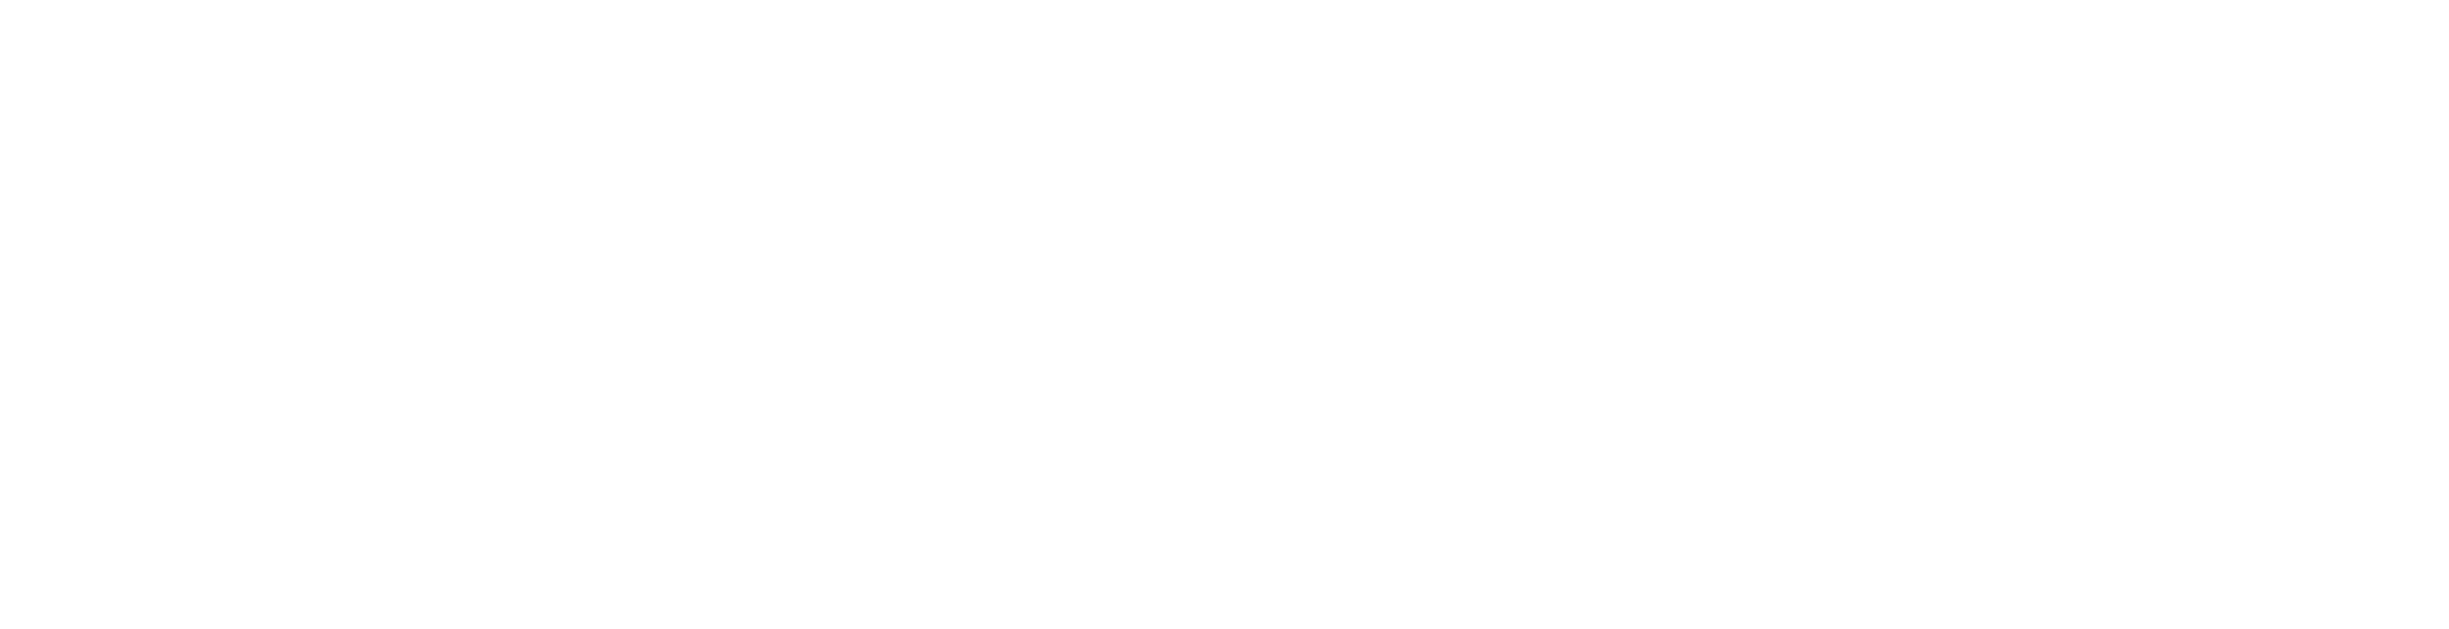
\includegraphics[height=2em]{logos/transp.png}}
\logoleft{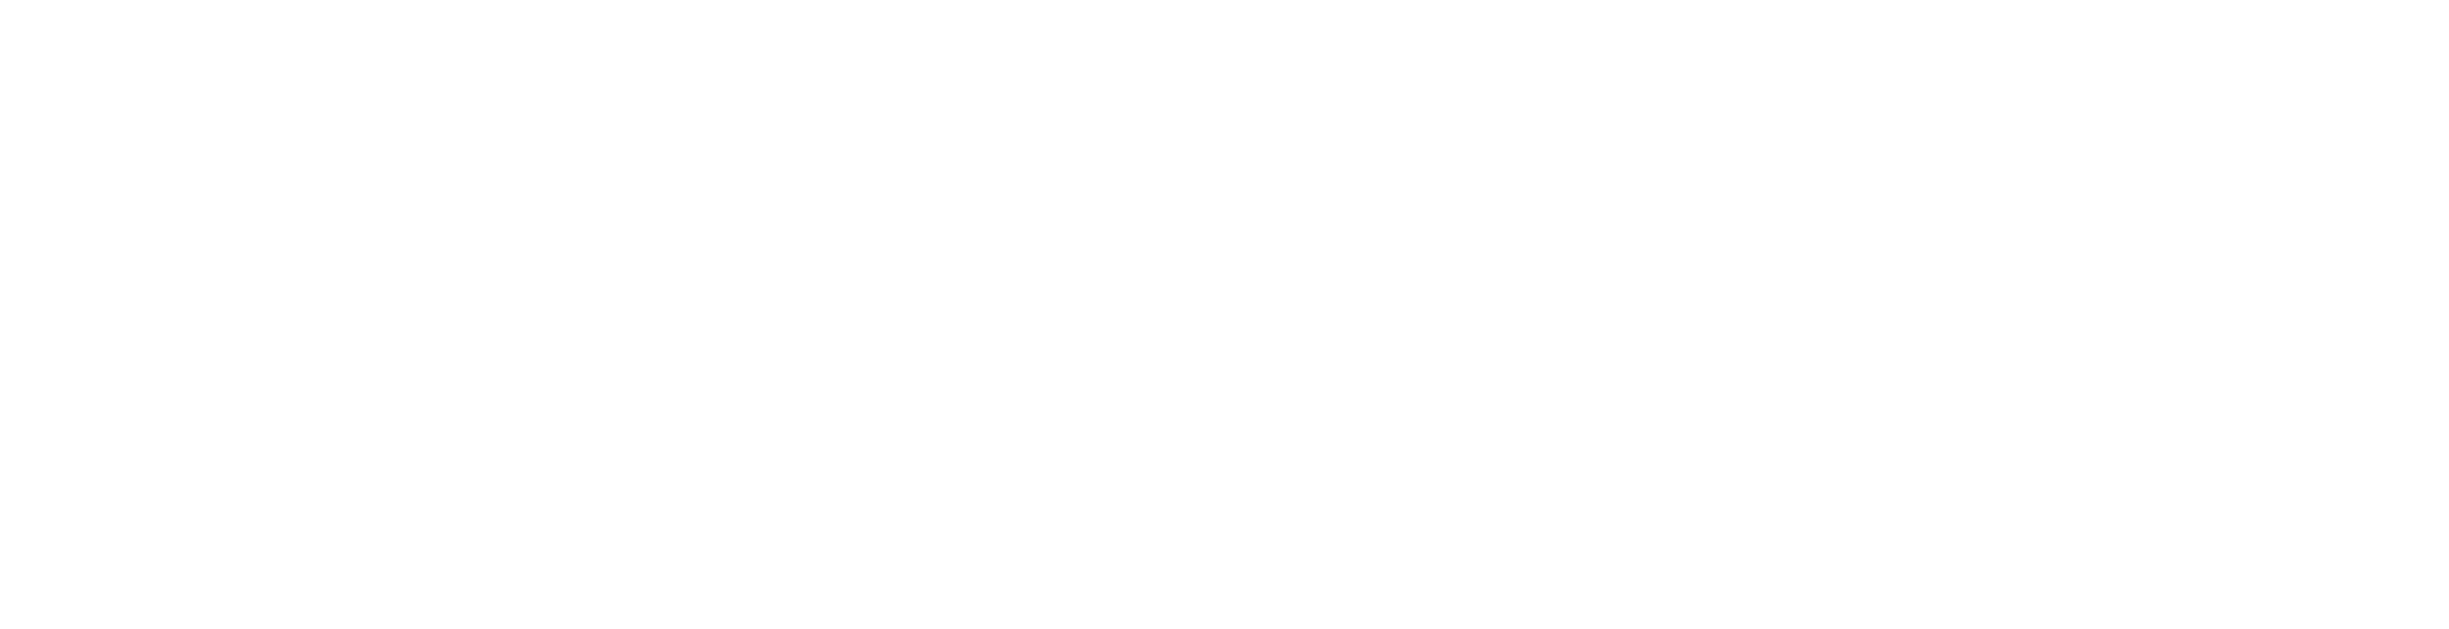
\includegraphics[height=2em]{logos/transp.png}}

% ====================
% Body
% ====================

\begin{document}

% Refer to https://github.com/k4rtik/uchicago-poster
% logo: https://www.cam.ac.uk/brand-resources/about-the-logo/logo-downloads
% \addtobeamertemplate{headline}{}
% {
%     \begin{tikzpicture}[remember picture,overlay]
%       \node [anchor=north west, inner sep=3cm] at ([xshift=-2.5cm,yshift=1.75cm]current page.north west)
%       {\includegraphics[height=7cm]{logos/unott-logo.eps}}; 
%     \end{tikzpicture}
% }

\begin{frame}[t]
\begin{columns}[t]
\separatorcolumn

\begin{column}{\colwidth}

  \begin{block}{Background}

    \begin{itemize}
        \item \textbf{Kidney transplantation (KT)}: recognised as the best treatment for \textbf{end-stage chronic renal disease}
        \begin{itemize}
            \setlength{\itemindent}{1em}
            \item \textbf{Graft shortage} in countries with aging population

            \textbf{\textcolor{nottblue}{$\Rightarrow$ Necessity for expansion of graft pool}}
        \end{itemize}
        \item Wide use of \textbf{marginal grafts} with suboptimal properties for patient-graft survival
        \item Decision making tools to assist clinicians in evaluating graft proposals
        \begin{itemize}
            \setlength{\itemindent}{1em}
            \item \textbf{ECD \cite{metzger2003expanded}} Older than 60 years old or between 50 and 59 with at least 2 comorbidities among: high serum creatinine, history of hypertension and death by CVA
            
            \textbf{\textcolor{nottblue}{$\Rightarrow$ Binary criterion, no gradient between less and more marginal donors}}       
            \item \textbf{KDRI/KDPI \cite{rao2009comprehensive}} Continuous/percentile scale defined by 10 donor features
            
            \textbf{\textcolor{nottblue}{$\Rightarrow$ Not adapted to the french population \cite{dantan2021covariates} and prone to increased graft refusal rate \cite{aubert2019disparities}}}

        \end{itemize}
    \end{itemize}

\vskip-0.5em

{\centering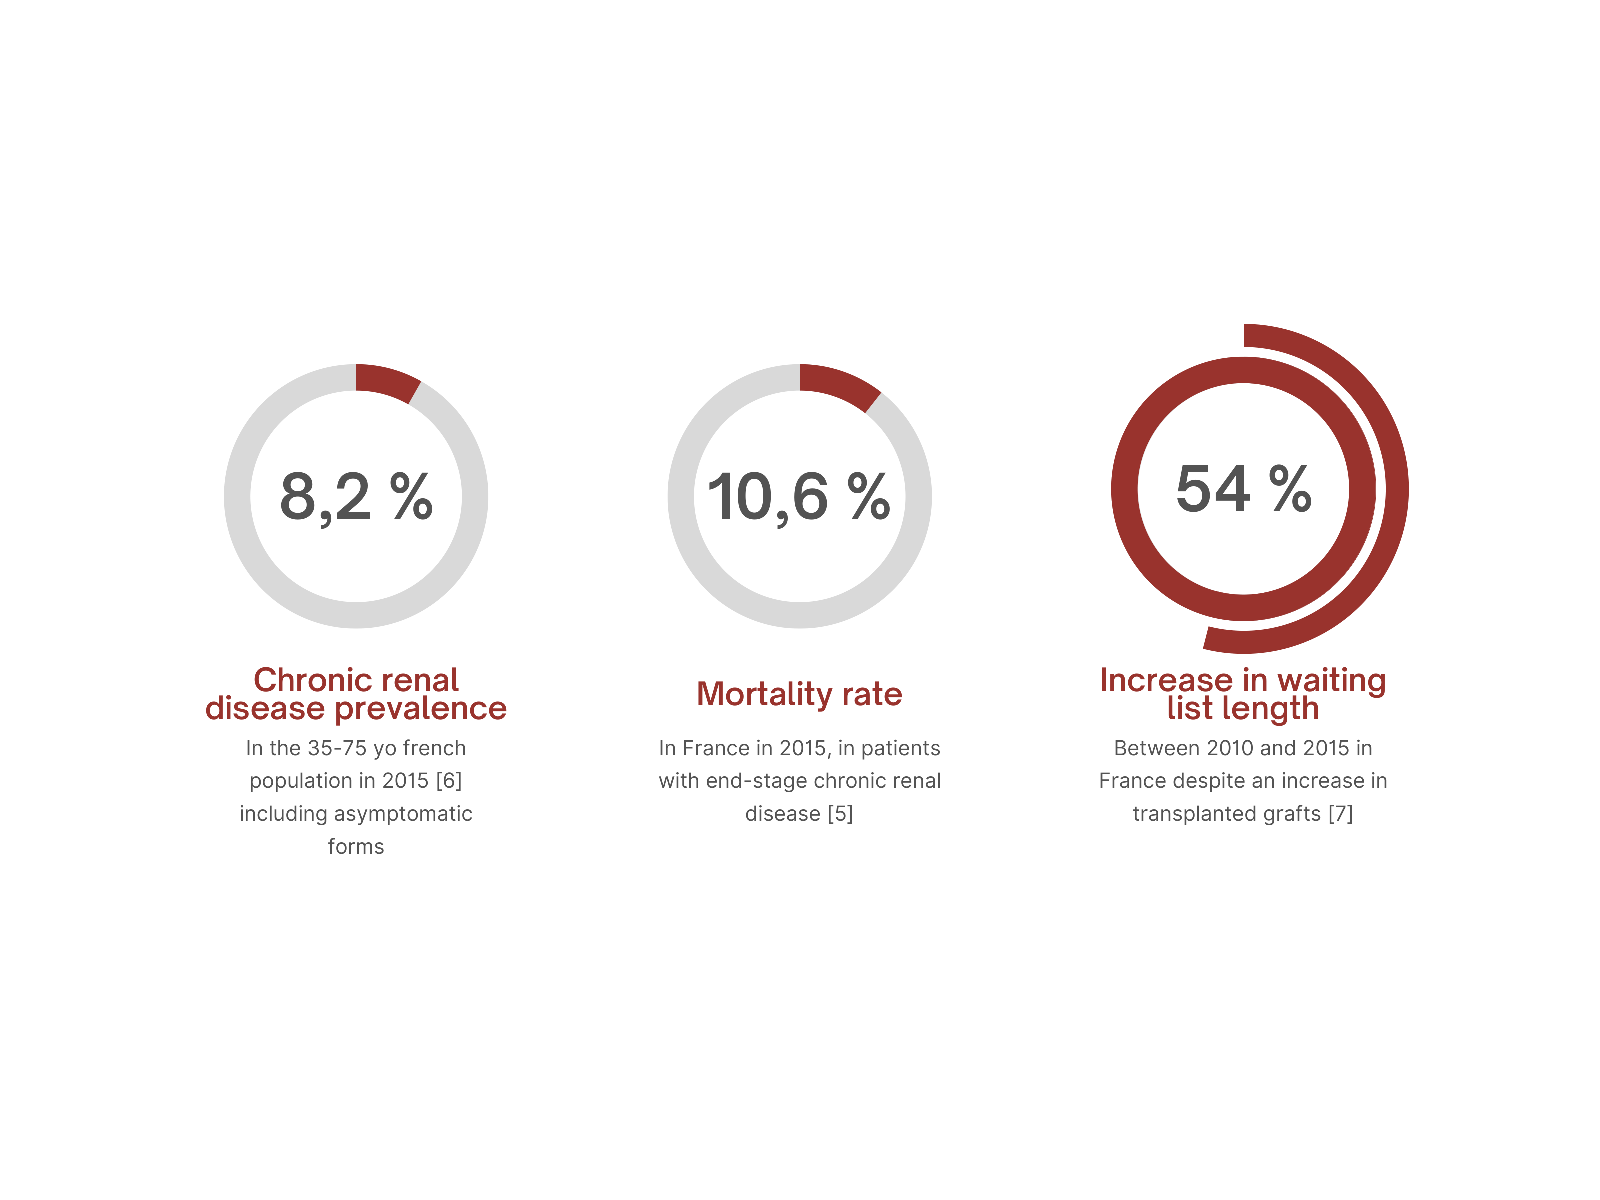
\includegraphics[scale=1.6]{Images/Chronic renal disease prevalence.pdf}\par}
    
\vskip-1em

  \end{block}




  \begin{block}{Objectives}

    Develop and validate a \textbf{\textcolor{nottblue}{kidney donor marginality score}}, \textbf{adapted to the french population} and \textbf{suited for the current practices} in KT in France

    \begin{itemize}
      \item \textbf{Donor/recipient interactions} will be studied in order to express donor marginality in relation to recipient characteristics
      \item \textcolor{darkgray}{\textbf{Recipient loss-of-chance} related to receiving a marginal graft as defined by the proposed score will be studied}
    \end{itemize}

  \end{block}

\begin{alertblock}{Materials and Methods}
    \begin{itemize}
        \item \textbf{7622 patients} from the DIVAT national kidney transplant cohort
        \item First-time deceased donor graft recipients without donor-recipient ABO incompatibility
        \item \textbf{Multivariate Cox regression} model built via blockwise variable selection approach (Donor/Graft/Recipient features integrated/removed from the model in 11 steps)
        \item Assessment of \textbf{period/center effect} via adjusted and frailty models
        \item New variable selection steps after integration of period/center effects
    \end{itemize}
        {\centering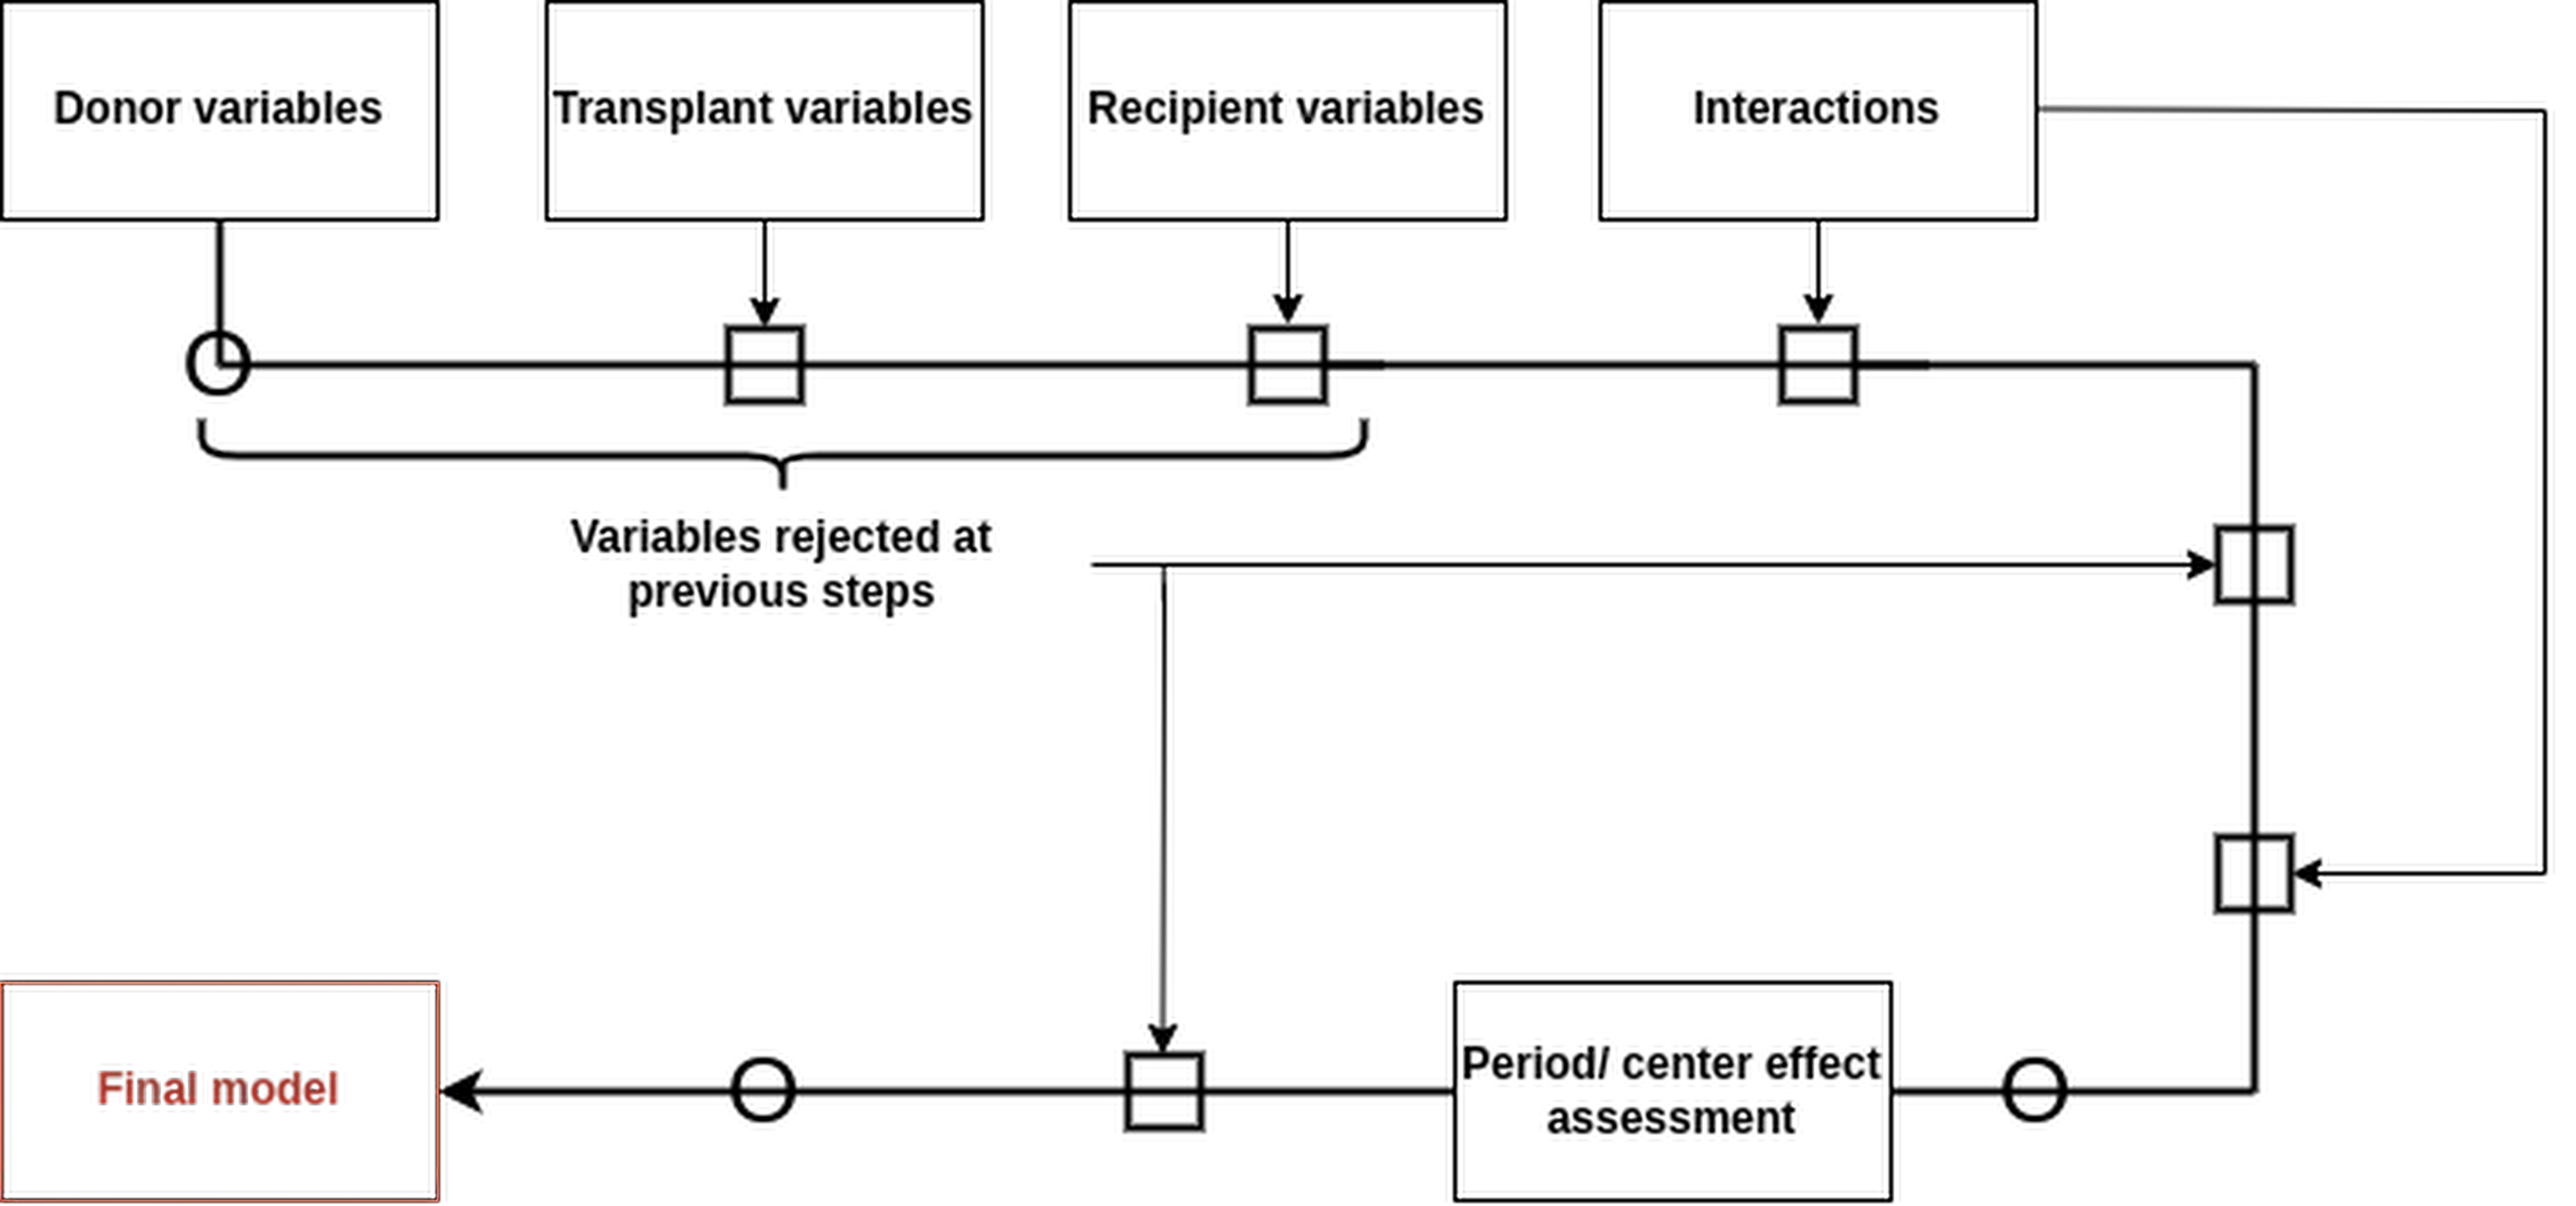
\includegraphics[scale=0.36]{Images/analyse.png}\par}
        {\centering\small \textbf{Variable selection process} (square nodes indicate all previously included predictors were forced in the model during backward selection, circle nodes indicate no variable was forced)\par}
        

    
  \end{alertblock}

\begin{block}{Funding}
\centering
    This work was supported by the French Biomedicine Agency (reference: AOR Greffe 2022) 
\end{block}


\vskip-0.15em
  \begin{block}{}
    {\centering
\includegraphics[scale=0.8]{logos/logband.png}\par}
  \end{block}

\end{column}

\separatorcolumn

\begin{column}{\colwidth}

  \begin{block}{Results}

\vskip-1em
  
\begin{figure}
    \centering
    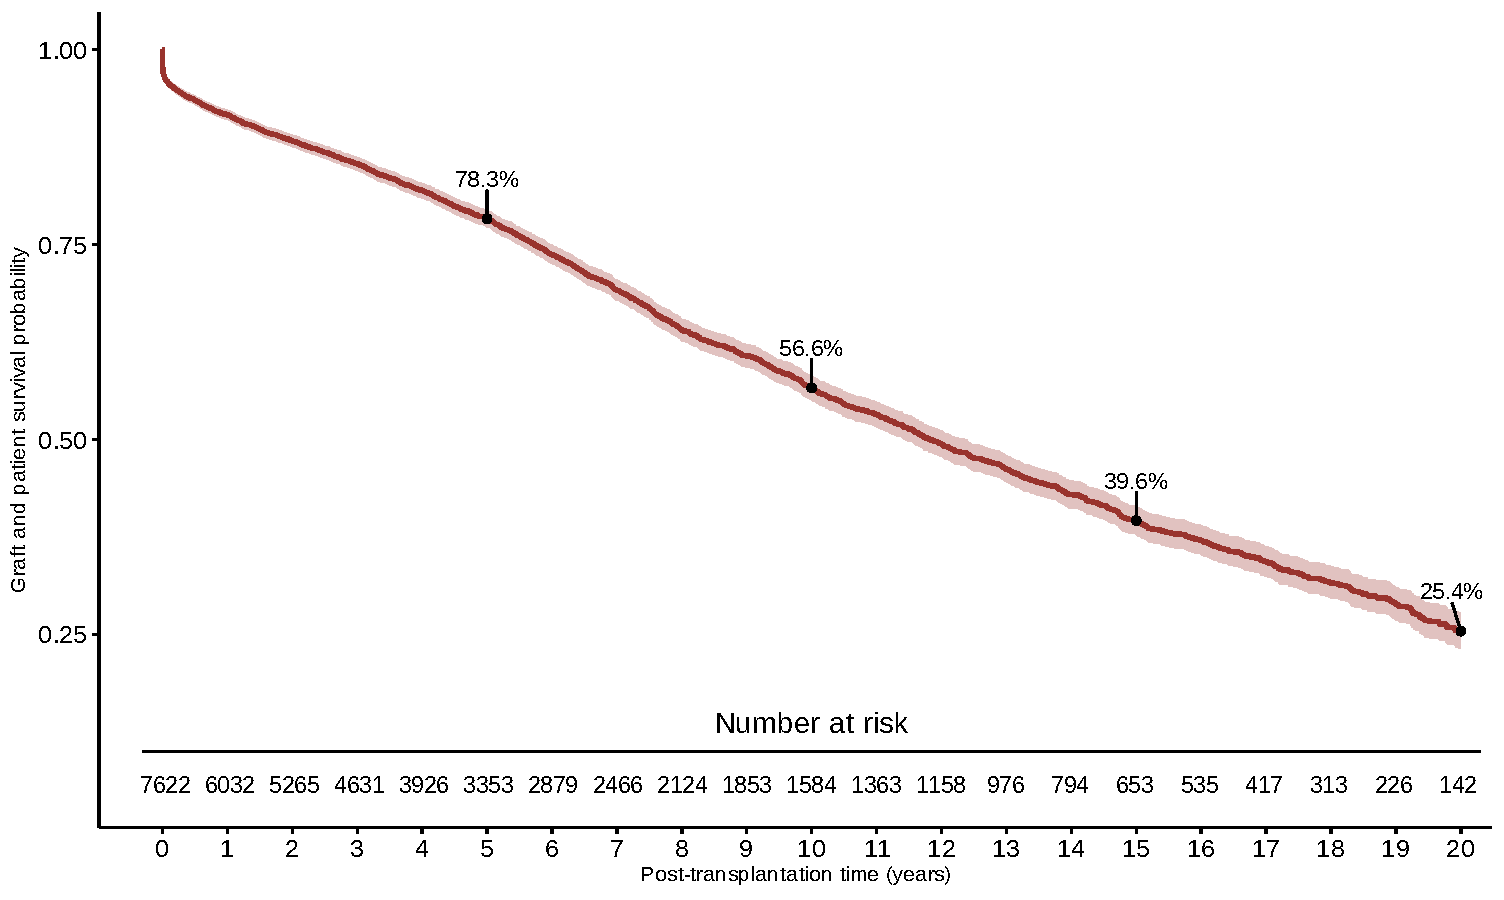
\includegraphics[scale=1.5]{Images/km_global.pdf}
    \vskip-1.25em
    \caption{Patient/allograft survival analysis}
    \label{fig:km}
\end{figure}



\begin{table}[]
\centering
\begin{tabular}{@{}lcccc@{}}
\toprule
                                            & \beta  & 95\% CI                  \\ \midrule
Donor age                                   & -0.020 & {[-0.037}-- {-0.003]}                    \\
Donor after cardiac death                   & 0.691  & {[0.416}--{0.967]}  \\
Donor death by CVA                          & -0.616 & {[-1.224}-- {-0.008]}                    \\
Donor serum creatinine                            & 0.001  & {[0.0001}--{0.002]}             \\
Donor height                                & -0.011 & {[-0.018}-- {-0.004]}             \\
Donor weight                                & 0.005  & {[0.001}--{0.010]}             \\
Positive donor CMV serology                 & 0.124  & {[0.010}--{0.239]}              \\
\addlinespace\addlinespace
\textcolor{darkgray}{\textbf{HLA incompatibilities \geq 4}}      & 0.151  & {[0.009}--{0.293]}             \\
Time on dialysis                            & 0.0001 & {[0.0001}--{0.0001]}            \\
Transplanted before 2012                    & 0.190  & {[0.040}--{0.340]}           \\
\addlinespace\addlinespace
Recipient age                               & -0.021 & {[-0.036}-- {-0.005]}                    \\
Recipient BMI                               & 0.011  & {[-0.003}--{0.025]}             \\
Recipient history of diabetes               & 0.376  & {[0.234}--{0.517]}  \\
Recipient history of cardiovascular disease & 0.408  & {[0.239}--{0.527]}  \\
Hemodialysis                                & 0.250  & {[0.048}--{0.452]}           \\
\textcolor{darkgray}{\textbf{Donor age*Recipient age}}                     & 0.001  &  {[0.0001}--{0.001]} \\
\textcolor{darkgray}{\textbf{Donor death by CVA*Recipient age}} & 0.014  &  {[0.003}--{0.024]}                   \\ \bottomrule
\end{tabular}
\caption{\label{mod-table}Proportional hazards Cox model analysis of retained factors and interactions after multivariate selection}
\end{table}

\vskip-1em

\begin{itemize}
    \item Donor age, beating heart status ($HR=2.00$), cause of death, creatininemia, height, weight and CMV serology ($HR=1.13$) will be integrated into the score. For a given donor, the score will differ depending on recipient age and donor/recipient HLA ABDR incompatibilities.
\end{itemize}

  \end{block}

\vskip-0.5em
  
  \begin{exampleblock}{What's next}
  \vskip0.3em
    \begin{itemize}
        \item \textbf{Internal validation} of the model, $\frac{1}{3}$ of the database allocated to a random validation sample

        \item \textbf{Validity assessed through:}
        \begin{itemize}
            \setlength{\itemindent}{1em}
            \item \textbf{Calibration:} calibration plot, predicted survival by score quantile, Brier score
            \item \textbf{Discrimination:} time-dependent ROC curve (AUC, PPV/NPV) and time-dependent ROC curve per recipient strata
        \end{itemize}
        \item \textbf{Propensity score}-based analysis to estimate population-averaged effects and propose a recipient loss-of-chance-based approach
        \item Development of an \textbf{online score computation tool} for clinicians
    \end{itemize}

  \end{exampleblock}

 \vskip-1em

  \begin{block}{References}
    \vskip-0.15em
    \nocite{*}
    \footnotesize{\bibliographystyle{plain}\bibliography{poster}}

  \end{block}


\end{column}
\separatorcolumn

\end{columns}
\end{frame}

\end{document}
